%-------------------------------------------------------------------------
% INFORMACIÓN DEL ARTÍCULO
\thispagestyle{portadapage}
\setcounter{subsection}{0}
\setcounter{subsubsection}{0}
\setcounter{actividad}{0}
\setcounter{actividad_previa}{0}
\setcounter{actividad_entre}{0}
\renewcommand{\articulotipo}{Taller}
\renewcommand{\articulotitulo}{Enseñanza del álgebra inicial a través de la modelización con un enfoque de la teoría antropológica didáctica}
\renewcommand{\articulotitulocorto}{Enseñanza del álgebra inicial a través de la modelización con un enfoque de la Teoría Antropológica Didáctica}
\section{\articulotitulo}
\desctotoc{Villagra, C.; Carrasco, R.; Alvarez, D.; Miguez, I.}

\noindent\rule{\linewidth}{2pt}

\vspace{0.25cm}

\begin{flushright}
	\addautor[villagracelia@gmail.com]{Celia Villagra}{Universidad Nacional de Salta}
	\vspace{1em}
	\addautor[]{Rosana Carrasco}{Universidad Nacional de Salta}
	\vspace{1em}
	\addautor[]{Daniela Alvarez}{Universidad Nacional de Salta}
	\vspace{1em}
	\addautor[]{Isabel Miguez}{Universidad Nacional de Salta}
\end{flushright}

\vspace{0.5cm}

\begin{center}
	\begin{minipage}{0.75\linewidth} \small
		\textsc{Resumen}. ~
		Ante las dificultades que tienen los estudiantes del nivel medio para comprender los objetos del álgebra, surgen investigaciones como las de \textcite{gascon1999} y \textcite{bolea2003} que consideran que es necesaria una concepción procedimental del álgebra, haciendo hincapié en la modelización. Pero en la escuela secundaria es frecuente que la modelización en matemática esté restringida a la aplicación de conocimientos matemáticos, ya aprendidos, a situaciones reales o artificiales. La Teoría Antropológica de lo Didáctico (TAD), según \textcite{chevallard1999},  busca integrar los principios de la antropología y la didáctica para mejorar la educación matemática, reconociendo la importancia de la diversidad cultural, el contexto social y la participación activa de los estudiantes en el proceso de enseñanza-aprendizaje, por lo que promueve la construcción del sentido de los conceptos matemáticos. La TAD propone que toda actividad humana puede ser modelada mediante praxeologías, a partir  de esta idea   es que en el taller se propiciará la comprensión de los principios fundamentales de esta  teoría didáctica  y el análisis de diferentes propuestas de modelización que fueron diseñadas para la escuela Secundaria, particularmente en la construcción del Álgebra inicial.
	\end{minipage}\\
	
	\vspace{0.5em}
	
	\begin{minipage}{0.75\linewidth} \small
		\textsc{Palabras clave} --- Modelizacion matematica - TAD - Álgebra elemental - Enseñanza
	\end{minipage}
\end{center}
%-------------------------------------------------------------------------

\subsection{Introducción}

En la educación matemática del nivel secundario es frecuente que estudiantes se refieran a la poca aplicabilidad de los contenidos matemáticos y pregunten para qué sirve lo que se les enseña. Cuando se trata de la enseñanza inicial del álgebra tienen dificultades para la comprensión conceptual de los objetos fundamentales de esta rama de la matemática, que se pone de manifiesto en los errores que presentan cuando resuelven situaciones algebraicas. Es por ello que diferentes autores han pensado la matemática como una actividad de modelización lo que impulsa a un cambio de mirada sobre el trabajo que los docentes propician sobre sus estudiantes respecto al saber matemático. En la escuela media la modalización está generalmente restringida a la aplicación de conocimientos matemáticos, ya aprendidos, a situaciones reales o artificiales. La teoría antropológica de lo didáctico (TAD), propuesta por \textcite{chevallard1999}, busca integrar los principios de la antropología y la didáctica para mejorar la educación matemática, reconociendo la importancia de la diversidad cultural, el contexto social y la participación activa de los estudiantes en el proceso de enseñanza-aprendizaje, por lo que promueve la construcción del sentido de los conceptos matemático, proponiendo que toda actividad humana puede ser modelada mediante praxeologías. Recuperando los aportes de esta teoría didáctica en el taller se propiciará la comprensión de las nociones fundamentales de la TAD y el análisis de diferentes propuestas de modelización que fueron diseñadas para la escuela Secundaria, particularmente en la construcción del Álgebra elemental. Se busca que el docente sea capaz de reformular lo que entiende por procesos de modelización y que se inicie en el diseño de problemas incorporando diferentes tipos de praxeologías para propiciar la construcción de sentido del álgebra elemental en sus estudiantes.

\subsection{Contenidos}

Modelización en Matemática. Concepciones. La modelización en matemática según diferentes escuelas didácticas. Teoría Antropológica didáctica. Praxeología. Tradiciones en la enseñanza del álgebra. Enseñanza del álgebra a partir de situaciones de modelización.

\subsection{Requisitos previos}

Tener conocimientos de herramientas básicas de GeoGebra. Dominio sobre los
contenidos de álgebra que se enseñan en la escuela secundaria.

\subsection{Objetivos}

\begin{itemize}
	\item Reformular la concepción de modelización privilegiando la construcción de 	sentido como idea fundamental.
	\item Comprender los principios básicos de la Teoría Antropológica Didáctica.
	\item Valorar la construcción de sentido de los objetos iniciales del álgebra en sus estudiantes a través de la incorporación de problemas de diferentes praxeologías.
\end{itemize}

\subsection{Actividades}

\subsubsection{Actividades previas}
\begin{enumerate}
	\item Los asistentes al taller deberán completar una encuesta para indagar acerca de las concepciones que tienen sobre modelización en matemática. Se adjunta el enlace del formulario en Google que deberán completar \url{https://forms.gle/gCoNxXTbzK4hfzHM7}
	
	\item Los docentes deberán mirar un video de Patricia Sadovsky que se encuentra en el siguiente enlace \url{https://youtu.be/W0ZocU8f-sc?si=vGea6gBz1TZfOdVE} y responder las siguientes preguntas:
	
	\begin{enumerate}[2.1]
		\itshape
		\item ¿En qué se diferencia la enseñanza de la matemática desde sus inicios en la Escuela Secundaria con respecto a la actualidad?
		\item ¿De qué otros factores consideras que depende la efectividad o el resultado de la implementación de las estrategias didácticas aplicadas en la enseñanza de la matemática (condiciones institucionales o sociales)?
		\item ¿Cuál es el mayor desafío que enfrentas al construir sentido de las matemáticas en el aula?
		\item ¿Qué dificultades encuentras al establecer conexiones entre las herramientas que provee la matemáticas y los problemas que permite abordar?
		\item ¿Consideras que establecer conexiones entre las herramientas que ofrece la matemática y los problemas de la vida real, hace que los alumnos se involucren y les resulte más atractiva las matemáticas?
		\item ¿Qué tipo de consignas crees que deben plantearse para poder captar el aprendizaje de tus alumnos,
		\item ¿Crees que se puede estandarizar algún tipo de evaluación dirigida a probar algunos conocimientos en matemática?
		\item ¿Qué metodología utilizas para la enseñanza de la Matemática en tu práctica docente?
		\item ¿Qué opinas sobre la siguiente frase? Justifica.
		\begin{quote}
			"La enseñanza y el aprendizaje es un hecho esencialmente interactivo: No se puede enseñar si no hay alumnos y los alumnos no pueden aprender si no hay un mediador, un docente que enseñe".
		\end{quote}
	\end{enumerate}
\end{enumerate}

\subsubsection{Primera hora y media sincrónica}

\begin{enumerate}
	\item Actividad grupal. Los asistentes deberán analizar dos actividades, una de ellas corresponde a una situación de modelización según la concepción que nos interesa.
	\item Se realizará la puesta en común de las actividades anteriores
	\item Un tallerista presenta las diferentes concepciones de modelización. Se referirá de manera particular a la modelización como metodología de enseñanza.
	\item Se analizará la actividad de modelización resuelta propiciando la discusión sobre la concepción de modelización subyacente y los pasos que puede llevar a cabo el docente para trabajarla en el aula.
\end{enumerate}

\begin{center}
	\begin{minipage}{0.7\linewidth}
		\paragraph*{Actividad propuesta “Planes de Ahorro”}
		
		\begin{enumerate}[{Consigna} 1:]
			\item Analizar la actividad propuesta a estudiantes.
			\item Identificar contenidos involucrados
			\item Proponer tareas que puede llevar a cabo el estudiante para tomar la decisión sobre el plan de ahorro adecuado.
		\end{enumerate}
	\end{minipage}
\end{center}

\bigskip

\begin{quote}
	\itshape
	"Deseamos planear con tiempo el viaje de fin de curso, para lo que tenemos que decidir un plan de ahorro que nos permita reunir una cantidad suficiente de dinero. Aunque no sabemos aún el precio exacto del viaje, podemos hacer una estimación de la cantidad de dinero que necesitamos, y comenzar a tomar decisiones sobre los diferentes plazos de entrega, las diferentes cantidades a dar en cada plazo, etc. Por supuesto, no se trata de decidir hoy cuánto dinero hay que entregar y cómo, sino de empezar a trabajar sobre ello, con la intención de anticiparnos a final de curso y a las necesidades que tendremos cuando sepamos el precio exacto del viaje.” (García, 2005, p. 365)
\end{quote}

\subsubsection{Primeras tres horas entre clases}

\begin{enumerate}
	\item Se les solicitará a los asistentes al taller que miren un video que se incrustará en la página Moodle \url{https://youtu.be/xbsQN6AFPCY?si=Sbpv8mV\_vrBw--J5}
	
	\bigskip
	\begin{minipage}{0.9\linewidth}
		\textit{Completar}
		
		\begin{itemize}
			\item La Teoría Antropológica de lo Didáctico (TAD) es el estudio del \_\_\_\_\_\_\_\_\_\_ en la \_\_\_\_\_\_\_\_\_\_ aplicado a la \_\_\_\_\_\_\_\_\_\_. Se fundamenta en la \_\_\_\_\_\_\_\_\_\_, que a su vez implica realizar un estudio de la \_\_\_\_\_\_\_\_\_\_, \_\_\_\_\_\_\_\_\_\_, \_\_\_\_\_\_\_\_\_\_ y \_\_\_\_\_\_\_\_\_\_.
			\item La estructura lógica del diseño curricular en el marco de la TAD, es un proceso
			que consta de \_\_\_\_\_\_\_\_\_\_ etapas bien diferenciadas.
			\item La primera etapa enfatiza que es necesario plantear al alumno una \_\_\_\_\_\_\_\_\_\_ que le resulte \_\_\_\_\_\_\_\_\_\_ y genere en él \_\_\_\_\_\_\_\_\_\_ de resolverlo. En esta etapa intervienen además dos conjuntos de personas: conjunto de \_\_\_\_\_\_\_\_\_\_ y conjunto de \_\_\_\_\_\_\_\_\_\_.
			\item En la segunda fase, el alumno debe ser capaz de identificar \_\_\_\_\_\_\_\_\_\_ cuestiones problemáticas (subproblemas) que se derivan o están relacionadas con el \_\_\_\_\_\_\_\_\_\_ inicial y que necesitan ser abordadas a los efectos de \_\_\_\_\_\_\_\_\_\_.
			\item En la tercera etapa el alumno propone posibles \_\_\_\_\_\_\_\_\_\_ a cada uno de los subproblemas planteados en la etapa anterior, obtenidas mediante la consulta de diferentes \_\_\_\_\_\_\_\_\_\_. Es decir, formula respuestas \_\_\_\_\_\_\_\_\_\_ que lo ayudarán a construir una respuesta \_\_\_\_\_\_\_\_\_\_.
			\item En el cuarto paso, se configura un \_\_\_\_\_\_\_\_\_\_ \_\_\_\_\_\_\_\_\_\_, formado por los siguientes elementos \_\_\_\_\_\_\_\_\_\_, \_\_\_\_\_\_\_\_\_\_, \_\_\_\_\_\_\_\_\_\_ y \_\_\_\_\_\_\_\_\_\_.
			\item En el último paso se elabora una \_\_\_\_\_\_\_\_\_\_ tentativa y \_\_\_\_\_\_\_\_\_\_ del \_\_\_\_\_\_\_\_\_\_ inicial.
		\end{itemize}
	\end{minipage}
	\bigskip
	
	\item  Deberán resolver el problema Planes de Ahorro, utilizando la planilla de cálculo de GeoGebra o de Excel y analizarlo teniendo en cuenta algunas ideas fundamentales de la TAD expresadas en el video anterior.
\end{enumerate}

\subsubsection{Segundas hora y media sincrónicas}

\begin{enumerate}
	\item Se recuperará la actividad resuelta en las horas entre clases.
	\item Un tallerista explicará los principios básicos de la TAD y su vinculación con la modelización.
	\item En grupos resolverán la siguiente actividad diseñada por Banchio (2021)
	
	\begin{actividad}
		Dado un paralelogramo, ¿es posible inscribirlo en una circunferencia de radio $r$? Si es así, ¿existe una relación de dependencia entre el área del paralelogramo y el radio $r$? ¿Y entre el perímetro y el radio? Entre todos los paralelogramos inscriptibles, ¿Existirá uno de mayor área? ¿Y uno de mayor perímetro?
	\end{actividad}
	
	\item Puesta en común de la resolución de la actividad
	\item Discusión respecto al valor didáctico de la actividad en el marco de la modelización de la TAD.
\end{enumerate}

\subsubsection{Segundas tres horas entre clases}

Análisis de una propuesta de modelización en la que deben responder:
\begin{enumerate}[a]
	\item ¿En qué contexto está la situación?
	\item ¿Es una actividad de modelización? ¿por qué?
	\item ¿Qué contenidos están involucrados?
	\item ¿Cuál es el valor didáctico de la actividad?
	\item Diseñe con GeoGebra el ítem 2 y suba el archivo generado. ¿Cuál es la importancia de poder resolver la actividad usando GeoGebra?
\end{enumerate}

\bigskip

\begin{center}
	\begin{minipage}{0.8\linewidth}
		\textbf{Situación 1: El cuadrado que cumple años}. Propuesta por \textcite{audisio2019}
		
		\begin{enumerate}
			\item Tenemos un cuadrado que tiene un año de edad y mide $1 \text{cm}^2$. ¿Cómo será el cuadrado cuando cumpla dos años de edad, si de un año al siguiente su lado aumenta en $1 \text{cm}^2$? Si tomamos un cuadrado de $1 \text{cm}$ como unidad, ¿cuántos cuadrados unidad tendrá el Cuadrado a los dos años?
			\item Supongamos que el Cuadrado, al ir creciendo, mantiene el contorno pintado de rojo. ¿Cómo será el Cuadrado a los 3, 4, 5 y 10 años?. Organice los datos que obtenga al responder las siguientes preguntas:
			\begin{enumerate}[a]
				\item ¿Qué longitud tiene el lado del cuadrado?
				\item ¿Cuál es el perímetro del cuadrado cuando va cumpliendo años?
				\item Mida el área del cuadrado
				\item ¿Cuántos cuadrados unidad de los que forman la figura tienen dos lados pintados?
				\item ¿Cuántos cuadrados unidad de los que forman la figura tienen un lado pintado?
				\item ¿Cuántos cuadrados unidad de los que forman la figura no tienen ningún lado pintado?
				\item Encuentre una expresión que responda a los ítems anteriores para cuando el cuadrado tenga $n$ años
			\end{enumerate}
			
			\item Observe en la figura \ref{fig:grafico01}, los siguientes cubos formados cada uno de ellos por cubos de unidad.
			
			Consigne cuántos cubos unidad necesito para armar los cuerpos 1, 2, 3, 4, n. Si deseo pintar los cuerpos 1, 2, 3, 4, n, ¿a cuántos cubos unidad le pintaré sólo 1 de sus caras, a cuántos solo 2 de sus caras, a cuántos 3 de sus caras o ninguna cara?. Construya una tabla con los datos y establezca relaciones. Tenga en cuenta que el cuerpo 1 mide $1 \text{cm}^3$.
			
			Puede utilizar el applet Diseño de cuerpos geométricos en papel isométrico de la plataforma \url{http://illuminations.nctm.org/ActivityDetail.aspx?ID=125} para graficar los cuerpos de 4 a $n$.
		\end{enumerate}
	\end{minipage}
	
	\begin{figure}[h!]
		\centering
		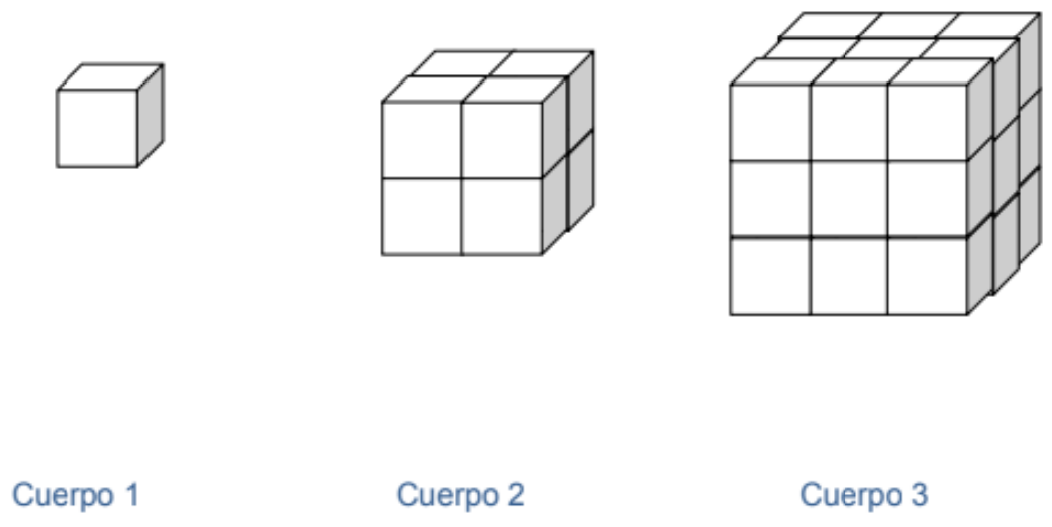
\includegraphics[width=0.7\linewidth]{Trabajos/04/Anexos/grafico_01.png}
		\caption{}
		\label{fig:grafico01}
	\end{figure}
\end{center}

\subsubsection{Terceras hora y media sincrónicas}

\begin{enumerate}
	\item Se retomará la actividad entre clases y se analizará cómo puede llevarse a cabo la gestión de la clase
	\item Se conformarán grupos para que cada uno resuelva una de las cinco actividades diseñadas en el documento “Matemática para la Formación	Docente” (\url{https://drive.google.com/file/d/1X_Hz86UvQZhWuBMkGTj9cY0JmMQt4Ia0/view?usp=sharing}) propuesto por Dirección de Educación Superior de la Provincia de Córdoba de la modelización con enfoque en la TAD.
	\item Puesta en común
	\item Recomendaciones finales por parte de los talleristas para trabajar el álgebra inicial a través de la modelización.
\end{enumerate}

\subsubsection{Evaluación final}

\begin{enumerate}
	\item  Se les proporcionará una actividad de modelización cuyo contenido principal será del álgebra inicial.
	\begin{enumerate}[{1}.1]
		\item Resuelva la actividad.
		\item Identifique el contexto de la situación planteada.
		\item Identifique los contenidos involucrados y el o los que se quiere enseñar.
		\item Justifique con marco teórico por qué corresponde a una actividad de modelación
		\item Exprese cómo gestionaría la clase
	\end{enumerate}
	
	\item En no menos de 4 líneas exprese una reflexión escrita sobre la experiencia del taller y el aprendizaje obtenido.
\end{enumerate}

\subsection{Bibliografía}

\nocite{*}
\printbibliography[keyword={04}]